% This is "sig-alternate.tex" V2.1 April 2013
% This file should be compiled with V2.5 of "sig-alternate.cls" May 2012
%
% ----------------------------------------------------------------------------------------------------------------
% This .tex file (and associated .cls V2.5) produces:
%       1) The Permission Statement
%       2) The Conference (location) Info information
%       3) The Copyright Line with ACM data
%       4) NO page numbers
%
% as against the acm_proc_article-sp.cls file which
% DOES NOT produce 1) thru' 3) above.
%
% Using 'sig-alternate.cls' you have control, however, from within
% the source .tex file, over both the CopyrightYear
% (defaulted to 200X) and the ACM Copyright Data
% (defaulted to X-XXXXX-XX-X/XX/XX).
% e.g.
% \CopyrightYear{2007} will cause 2007 to appear in the copyright line.
% \crdata{0-12345-67-8/90/12} will cause 0-12345-67-8/90/12 to appear in the copyright line.
%
% ---------------------------------------------------------------------------------------------------------------
% This .tex source is an example which *does* use
% the .bib file (from which the .bbl file % is produced).
% REMEMBER HOWEVER: After having produced the .bbl file,
% and prior to final submission, you *NEED* to 'insert'
% your .bbl file into your source .tex file so as to provide
% ONE 'self-contained' source file.
%
% For tracking purposes - this is V2.0 - May 2012

\documentclass{sig-alternate-05-2015}

\usepackage{graphicx}
\DeclareGraphicsExtensions{.pdf,.png}
\graphicspath{{./figures/}}

\begin{document}

% Copyright
\setcopyright{acmcopyright}
%\setcopyright{acmlicensed}
%\setcopyright{rightsretained}
%\setcopyright{usgov}
%\setcopyright{usgovmixed}
%\setcopyright{cagov}
%\setcopyright{cagovmixed}


% DOI
%\doi{10.475/123_4}

% ISBN
%\isbn{123-4567-24-567/08/06}

%Conference
%\conferenceinfo{PLDI '13}{June 16--19, 2013, Seattle, WA, USA}

%\acmPrice{\$15.00}

%
% --- Author Metadata here ---
%\conferenceinfo{WOODSTOCK}{'97 El Paso, Texas USA}
%\CopyrightYear{2007} % Allows default copyright year (20XX) to be over-ridden - IF NEED BE.
%\crdata{0-12345-67-8/90/01}  % Allows default copyright data (0-89791-88-6/97/05) to be over-ridden - IF NEED BE.
% --- End of Author Metadata ---

\title{Performance Monitoring and Root Cause Analysis for Cloud-hosted Web Applications}
\author{
% The command \alignauthor (no curly braces needed) should
% precede each author name, affiliation/snail-mail address and
% e-mail address. Additionally, tag each line of
% affiliation/address with \affaddr, and tag the
% e-mail address with \email.
%
% 1st. author
\alignauthor
Hiranya Jayathilaka, Chandra Krintz, Rich Wolski\\
       \affaddr{Computer Science Department}\\
       \affaddr{University of California, Santa Barbara}\\
       \email{\{hiranya,ckrintz,rich\}@cs.ucsb.edu}
}
\maketitle
\begin{abstract}
This paper provides a sample of a \LaTeX\ document which conforms,
somewhat loosely, to the formatting guidelines for
ACM SIG Proceedings. It is an {\em alternate} style which produces
a {\em tighter-looking} paper and was designed in response to
concerns expressed, by authors, over page-budgets.
It complements the document \textit{Author's (Alternate) Guide to
Preparing ACM SIG Proceedings Using \LaTeX$2_\epsilon$\ and Bib\TeX}.
This source file has been written with the intention of being
compiled under \LaTeX$2_\epsilon$\ and BibTeX.

The developers have tried to include every imaginable sort
of ``bells and whistles", such as a subtitle, footnotes on
title, subtitle and authors, as well as in the text, and
every optional component (e.g. Acknowledgments, Additional
Authors, Appendices), not to mention examples of
equations, theorems, tables and figures.

To make best use of this sample document, run it through \LaTeX\
and BibTeX, and compare this source code with the printed
output produced by the dvi file. A compiled PDF version
is available on the web page to help you with the
`look and feel'.
\end{abstract}

%
%  Use this command to print the description
%
\printccsdesc

% We no longer use \terms command
%\terms{Theory}

\keywords{ACM proceedings; \LaTeX; text tagging}

\section{Introduction}
\textbf{Cloud computing turns compute infrastructures, programming platforms and software systems
into online utility services that can be easily shared among many users~\cite{hassan2011demystifying,Mell:2011:SND:2206223}.}
It enables processing and storing data on large, managed infrastructures and 
programming platforms, that can be accessed remotely via the internet. This provides an
alternative to running applications on local servers, personal computers, and mobile devices,
all of which have strict resource constraints. 
Today, cloud computing technologies can be obtained from a large and growing number of providers.
Some of these providers offer hosted cloud platforms that can be used
via the web to deploy applications without installing any physical hardware 
(e.g. Amazon AWS~\cite{amazon-aws-web}, Google App Engine~\cite{gae}, Microsoft Azure~\cite{azure-web}). Others
provide cloud technologies as downloadable software, which users can install
on their computers or data centers to set up their own private clouds 
(e.g. Eucalyptus~\cite{eucalyptus09}, AppScale~\cite{6488671}, OpenShift~\cite{openshift}).

\textbf{Cloud computing model provides high scalability, high availability and enhanced levels of 
user productivity.} Cloud platforms run on large resource pools, typically in one or more
data centers managed by the platform provider. Therefore cloud platforms have access to a vast
amount of hardware and software resources. This enables cloud-hosted applications
to scale to varying load conditions, and maintain high availability. Moreover, by offering resources
as utility services, cloud computing is able to facilitate a cost-effective, on-demand
resource provisioning model that greatly enhances user productivity. 

\textbf{Over the last decade cloud computing technologies have enjoyed explosive growth, 
and near universal adoption due to their many benefits and 
promises~\cite{Antonopoulos:2010:CCP:1855007,Pinheiro:2014:ACC:2618168.2618188}.} 
Industry analysts project that the cloud computing market value will exceed \$150 billion
by the year 2020~\cite{cloud-growth}.
A large number of organizations
run their entire business as a cloud-based operation (e.g. Netflix, Snapchat). For startups
and academic researchers who do not have a large IT budget or a staff, the cost-effective 
on-demand resource provisioning model of the cloud has proved to be indispensable.
The growing number of academic conferences and journals dedicated to discussing
cloud computing is further evidence that cloud is an essential branch in the field
of computer science.

\textbf{Despite its many benefits, cloud computing has also given rise to several application
development and maintenance challenges that have gone unaddressed for many years.}
As the number of applications deployed in cloud platforms continue to increase these
shortcoming are rapidly becoming conspicuous. We highlight three such issues.
 
\textbf{Firstly, cloud platforms lack the ability to enforce developer best practices
and administrative conformance on deployed user applications.} The developer best practices 
are the result of decades of software engineering research, and
include code reuse, proper versioning of software artifacts, dependency management
between application components, and backward compatible software updates. Administrative
conformance refers to complying with various development and maintenance standards
that an organization may wish to impose on all of their production software.
Cloud platforms do not provide any facilities that enforce such developer practices or
administrative standards. Instead, cloud platforms
make it extremely trivial and quick to deploy new applications or update existing
applications (i.e. roll out new versions). The resulting speed-up of the development cycles combined with the lack of 
oversight and verification, makes it extremely difficult for 
IT personnel to manage large volumes of cloud-hosted applications.

\textbf{Secondly, today's cloud platforms do not provide support for establishing 
service level objectives (SLOs) regarding the performance of deployed applications.} 
A performance SLO specifies a bound on application's response time (latency). 
Such bounds are vital for developers 
who implement downstream systems that consume the cloud-hosted applications,
and cloud administrators who wish to maintain a consistent quality of service
level. However, when an application is implemented for
a cloud platform, one must subject it to extensive performance testing in order
to comprehend its performance bounds; a process that is both 
tedious and time consuming. The difficulty in understanding the performance 
bounds of cloud-hosted applications is primarily due to the very high level of 
abstraction provided by the cloud platforms. These abstractions shield many details 
concerning the application runtime, and without visibility into such low level application 
execution details it is impossible
to build a robust performance model for a cloud-hosted application. Due to this
reason, it is not possible to stipulate SLOs on the performance of cloud-hosted applications. 
Consequently, existing cloud platforms only offer SLOs regarding service availability.

\textbf{Thirdly, cloud platforms do not provide adequate support for monitoring application performance,
and running diagnostics when an application fails to meet its performance SLOs.} 
Most cloud platforms only provide the simplest monitoring and logging features,
and do not provide any mechanisms for detecting performance anomalies or identifying
bottlenecks in the application code or the underlying cloud platform. This limitation has given rise
to a new class of third party service providers that specialize in monitoring cloud applications
(e.g. New Relic~\cite{newrelic}, Dynatrace~\cite{dynatrace}, Datadog~\cite{datadog}). But these 
third party solutions are expensive. They also require code instrumentation, which
if not done correctly, leads to incorrect diagnoses. The perturbation
introduced by the instrumentation also changes and degrades application performance.
Furthermore, the extrinsic monitoring systems have a restricted view 
of the cloud platform, due to the high level of abstraction provided by cloud platform software.
Therefore they cannot observe the complexity of the cloud platform in full, and hence cannot pinpoint
the component that might be responsible for a perceived application performance anomaly.

\textbf{In order to make the cloud computing model more dependable, maintainable and convenient for the users as well
as the cloud service providers, the above limitations need to be addressed satisfactorily.}
Doing so will greatly simplify the tasks of developing cloud applications, and maintaining 
them in the long run. Developers will be able to specify SLOs on the performance of
their cloud-hosted applications, and offer competitive service level agreements (SLAs) to the end users that consume those
applications. Developers as well as cloud administrators will be able to detect performance anomalies
promptly, and take corrective actions before the issues escalate to major
outages or other crises.

\textbf{Our research focuses on addressing the above issues in cloud environments 
using \textit{governance}.} We define governance as the mechanism 
by which the acceptable operational parameters are specified and maintained in a 
software system~\cite{brown2005framing,gartner-soa-gov}. This involves multiple steps:
\begin{itemize}
\item Specifying the acceptable operational parameters
\item Enforcing the specified parameters
\item Monitoring the system to detect deviations from the acceptable behavior
\end{itemize}

To learn the feasibility and the efficacy of applying governance
techniques in a cloud platform, we propose and explore the following thesis
question:
{\bf Can we efficiently enforce governance for cloud-hosted web applications to achieve 
administrative conformance, developer best practices, and performance SLOs through 
automated analysis and diagnostics?} 

\textbf{For governance to be
useful within the context of cloud computing, it must be both efficient and automated.}
Cloud platforms are comprised of many components that have different life cycles
and maintenance requirements. 
They also serve a very large number of users who deploy applications in
the cloud. Therefore governance systems designed for the cloud should scale to handle a 
large number of applications and related software components,
without introducing a significant runtime overhead on them.
Also they must be fully automated since it is not practical for a human administrator to be
involved in the governance process given the scale of the cloud platforms.

Automated governance for software systems is a well researched area,
especially in connection with classic web services and service-oriented architecture 
(SOA) applications~\cite{gartner-soa-gov,soagov,Schepers:2008:LAS:1363686.1363932,5577268,4730489}. 
\textbf{We adapt the methodologies outlined in the existing SOA governance research corpus, so
they can be applied to cloud computing systems.}
These methodologies enable specifying
acceptable behavior via machine readable policies, which are then automatically enforced by
a policy enforcement agent. Monitoring agents watch the system to detect any deviations from
the acceptable behavior (i.e. policy violations), and alert users or follow predefined corrective
procedures. We can envision similar facilities being implemented in a cloud platform to 
achieve administrative conformance, developer best practices and performance SLOs. The operational
parameters in this case may include coding and deployment conventions for the cloud-hosted
applications, and their expected performance levels.

\textbf{In order to answer the above thesis question by developing efficient, automated governance systems,
we take the following three-step approach.}
\begin{itemize}
\item Design and implement a scalable, low-overhead governance framework for cloud platforms,
complete with a policy specification language and a policy enforcer. The governance framework should be
built into the cloud platforms, and must
keep the runtime overhead of the user applications to a minimum while enforcing
developer best practices and administrative conformance.
\item Design and implement a methodology for formulating performance SLOs (bounds)
for cloud-hosted web applications, without
 subjecting them to extensive performance testing or instrumentation. The formulated
SLOs must be correct, tight and durable in the face of changing conditions of the cloud.
 \item Design and implement a scalable cloud application performance monitoring (APM) framework for detecting
violations of performance SLOs. For each
violation detected, the framework should be able to run diagnostics, and identify the potential
root cause. It should support collecting data from the cloud platform
 without instrumenting user code, and without introducing significant runtime overheads.
\end{itemize}

\textbf{To achieve administrative conformance and developer best practices with minimal overhead,
we perform governance policy enforcement when an application is deployed; a technique that we
term deployment-time policy enforcement.} 
We explore the
trade off between what policies can be enforced, and when they can be enforced with respect
to the life cycle of a cloud-hosted application. We show that not all policies
are enforceable at deployment-time, and therefore some support for run-time policy enforcement
is also required in the cloud. However, we find that
deployment-time policy enforcement is efficient, and a governance framework that
performs most, if not all, enforcement tasks at deployment-time can scale
to thousands of applications and policies.

\textbf{We combine static analysis with platform monitoring to establish performance SLOs for
cloud-hosted applications.} Static analysis
extracts the sequence of critical operations (cloud services) invoked by a given application.
Platform monitoring facilitates constructing a historic performance model for the individual operations.
We then employ a time series analysis method to combine these results, and calculate statistical bounds 
for application response time. The performance bounds calculated in this manner
are associated with a specific correctness probability, and hence can be used
as SLOs. We also devise a statistical framework to evaluate the validity period of 
calculated performance bounds.

\textbf{In order to detect and diagnose performance SLO violations,
we monitor various performance events that occur in the cloud platform,
correlate them, and employ statistical analysis to identify anomalous patterns.} Any given statistical
method is only sensitive to a certain class of anomalies. Therefore, to be able to diagnose a wide range of
performance anomalies, we devise an algorithm that combines linear regression, change point
detection and quantile analysis. Our approach detects performance SLO violations in near real time,
and identifies the root cause of each event as a workload change or a performance bottleneck
in the cloud platform. In case of performance bottlenecks, our approach also correctly identifies
the exact component in the cloud platform, in which the bottleneck manifested.

\textbf{Our contributions push the state of the art in cloud computing significantly towards achieving
administrative conformance, developer best practices and performance SLOs.} Moreover,
our work addresses all the major steps associated with software system governance --
specification, enforcement and monitoring. We show that this approach can significantly improve cloud platforms
in terms of their reliability, developer-friendliness and ease of management. We also demonstrate
that the governance capabilities proposed in our work can be built into existing cloud platforms,
without having to implement them from the scratch.

\section{Background}
The popularization of network computing and the World Wide Web (WWW) 
has led to the development and adoption of web services~\cite{6094008} as
the technology of choice for implementing modern service-oriented 
architectures (SOA~\cite{Haines:2010:SAM:1787234.1787269}).
The interface portion of a web service, which abstracts and modularizes
its service implementation
details while making the service network-accessible, is commonly referred to
as a {\em web API}. As far as the users and applications that consume a 
web service
are concerned, the web API is the only point of contact and source of
functionality for the underlying service implementation.

Software engineering best practices separate the service implementation
from API, both during development and maintenance.
The service implementation and API are integrated via 
a ``web service stack'' that implements functionality common to all web
services (message routing, request authentication, etc.).
Because the API is visible to external parties ({\em i.e.} clients of the
services), any changes to the API
impacts users and applications not under the immediate administrative control
of the API provider.  For this reason, API features 
usually undergo long
periods of ``deprecation'' so that independent clients of the services can have
ample time to ``migrate'' to newer versions of an API.  On the other hand,
technological innovations often prompt service reimplementation and/or 
upgrade to
achieve greater cost efficiencies, performance levels, etc.
Thus, APIs typically have a more
slowly evolving and longer lasting lifecycle than the service
implementations to which they interface. 

Cloud computing is based on the idea of exposing some digital asset or a
capability ({\em e.g.} compute power, database, etc.) 
as a highly scalable web service.  Mobile
devices, due to their limited hardware resources often offload much of their
processing and storage needs to remote services running in a ``cloud''
connected to the Internet.  Web APIs
play a crucial role in both these paradigms. 

Consequently, modern computing clouds, especially clouds implementing some form
of Platform-as-a-Service (PaaS)~\cite{4548165}, have accelerated the
proliferation of web APIs and their use.  Most PaaS
clouds~\cite{appscale13,cloudfoundry,openshift} include
features designed to
ease the development and hosting of web APIs for scalable use over the Internet. 
This phenomenon is making API governance an absolute necessity in the cloud
environments.

In particular, API governance promotes code reuse among developers
since each API must be treated as a tracked and controlled software entity.
It also ensures that software users benefit from change control since the APIs
they depend on
change in a controlled and non-disruptive manner.  From a maintenance
perspective, API governance 
makes it possible to enforce best-practice coding procedures, 
naming conventions, and deployment procedures uniformly.
API governance is also critical to API lifecycle
management --  the management of deployed APIs in response to new feature
requests, bug fixes, and organizational priorities. 
API ``churn'' that results from lifecycle management
is a common phenomenon and a growing
problem for web-based applications~\cite{6930607}.
Without proper governance systems to manage the constant evolution of APIs,
API providers run the risk of making their APIs unreliable while potentially
breaking downstream applications that depend on the APIs.

Unfortunately, most web technologies used to develop and host web APIs do not 
provide API governance facilities. This missing functionality is
especially glaring
for cloud platforms that are focused on rapid
deployment of APIs at scale.   Commercial pressures frequently prioritize
deployment speed and scale over longer-term maintenance considerations only to
generate unanticipated future costs.

As a partial countermeasure, developers of cloud-based web services are 
frequently given
additional tasks associated with 
implementing custom {\em ad hoc} governance solutions using either locally
developed mechanisms or loosely integrated
third-party API management services. 
These add-on governance
approaches often fall short in terms of their consistency and enforcement
capabilities since
by definition they have to operate outside the
cloud (either external to it or as a cloud-hosted application). 
As such, they do not have the end-to-end 
access to all the metadata and cloud-internal control mechanisms
that are necessary to implement strong governance at scale. 

\section{Architecture}
Roots is a holistic system for application performance monitoring (APM), 
performance anomaly detection, and root cause analysis.
It is operated by the cloud providers as a builtin PaaS service that collects data from
all the cloud components user applications interact with. Data collection, storage
and analysis all take place within the cloud, and the insights gained are communicated
to both the cloud administrators and application developers as needed.
The key intuition behind Roots is that, as an intrinsic PaaS service, Roots
has visibility into all activities of the PaaS cloud, across layers.
Moreover, since the PaaS applications we have observed spend most of their time in 
PaaS kernel services~\cite{Jayathilaka:2015:RTS:2806777.2806842}, we hypothesize
that we can infer application performance from observations of how
 the application uses the platform, i.e. by efficiently monitoring the time spent in 
PaaS kernel services. If we are able to do so, then we can avoid application
instrumentation and its downsides while detecting performance anomalies and 
identifying their root cause in near real time with low overhead.

The PaaS model that we assume with Roots is one 
in which the clients of a web application engage in a
``service-level agreement'' (SLA)~\cite{Keller:2003:WFS:635430.635442}
with the ``owner'' or operator of the application that is hosted in a PaaS cloud.  The SLA
stipulates a response-time ``service-level objective'' (SLO) that, if violated, 
constitutes a breech of the agreement.
If the performance of an application deteriorates to the
point that at least one of its SLOs is violated, we treat it 
as an \textit{anomaly}. Moreover, we refer to the process
of diagnosing the reason for 
an anomaly as \textit{root cause analysis}.
For a given anomaly, the root cause could be a change in the application workload or
a \textit{bottleneck} in the application runtime. Bottlenecks may occur in the 
application code, or in the PaaS kernel services that the application relies on.

Roots collects performance data across the cloud platform stack, and aggregates it based on 
request/response.  It uses this data to infer application performance, and to identify
SLO violations (performance anomalies).  Roots can further handle different types of anomalies
in different ways.  We overview each of these functionalities in the remainder of this section.

\subsection{Data Collection and Correlation}

We must address two issues when designing a monitoring framework for
a system as complex as a PaaS cloud.
\begin{enumerate}
\item Collecting data from multiple different layers.
\item Correlating data collected from different layers.
\end{enumerate}

%Any PaaS APM must (i) collect data from all layers of the PaaS software stack, and
%(ii) correlate related events across layers.
Each layer of the cloud platform is only able to collect data regarding the
state changes that are local to it. A layer cannot monitor state changes
in other layers due to the level of encapsulation provided by layers. However,
processing an application request involves cooperation of multiple layers. 
To facilitate system-wide monitoring and
bottleneck identification, we must gather data from all the different layers involved
in processing a request. To combine the information across layers
we correlate the data, and link events related to the same request together.

To enable this, we augment the front-end server of the cloud platform. 
Specifically, we have it tag incoming application requests with unique identifiers.
This request identifier is added to the HTTP request as a header, which is visible to all 
internal components of the PaaS cloud. Next, we configure data collecting agents 
within the platform to record the request identifiers along with any events they capture. 
This way we record the relationship between application requests, and the resulting
local state changes in different layers of the cloud, without breaking the existing level
of abstraction in the cloud architecture. This approach is also scalable, since the events are
recorded in a distributed manner without having to maintain any state at the data collecting agents. 
Roots aggregates the recorded events by request 
identifier to efficiently group the related events as required during analysis.

\begin{figure}
\centering
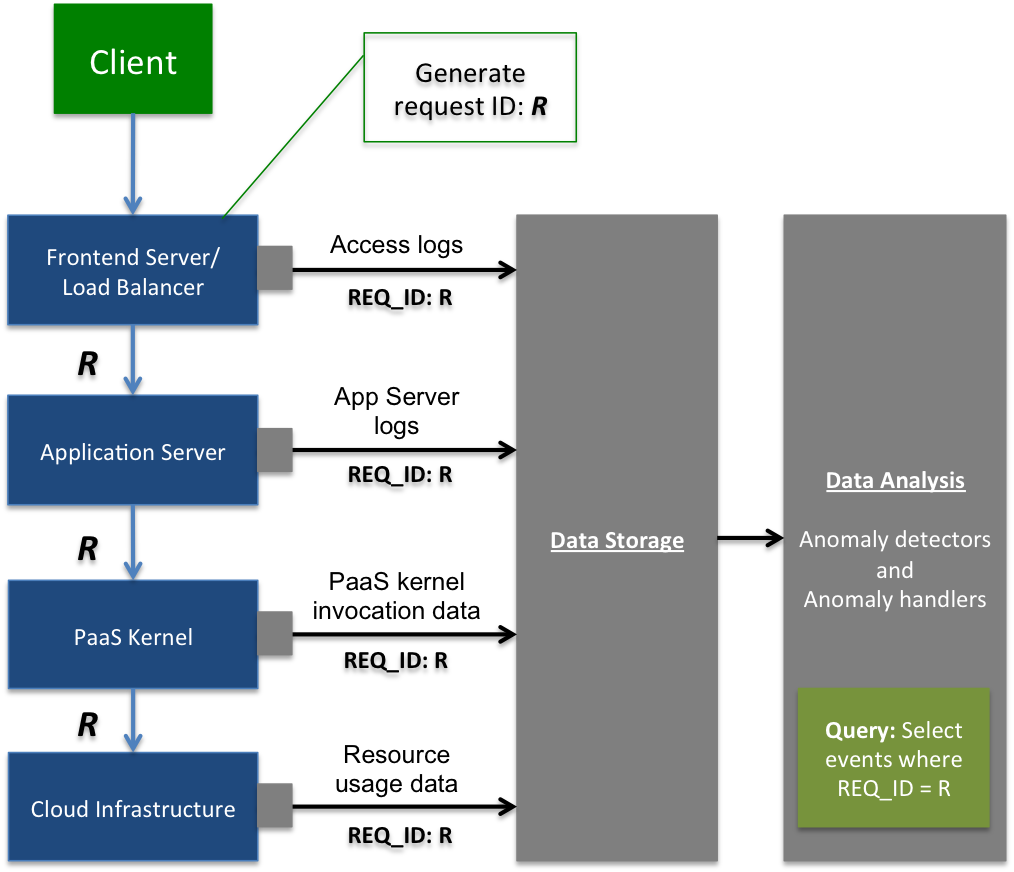
\includegraphics[scale=0.5]{apm_architecture}
\caption{Roots APM architecture.}
\label{fig:apm_architecture}
\end{figure}

Figure~\ref{fig:apm_architecture} illustrates the high-level architecture of Roots, and how 
it fits into the PaaS stack. APM components are shown in grey. 
The small grey boxes attached to the PaaS components represent the
agents used to instrument the cloud platform. 
In the diagram, a user request is tagged with the identifier value
$R$ at the front-end server. This identifier is passed down to the lower layers of the cloud
along with the request. Events that occur in the lower layers while processing this request
are recorded with the request identifier $R$, so Roots can correlate them later. For example, in the 
data analysis component we can run a filter query to select all the events related to a particular
request (as shown in the pseudo query in the diagram). Similarly, Roots can run a ``group by'' 
query to select all events, and aggregate them by the request identifier.

Figure~\ref{fig:apm_architecture} also
depicts Roots data collection across all layers in the 
PaaS stack (i.e. full stack monitoring). 
From the front-end server layer we gather information related to incoming application
requests. This involves scraping the HTTP server access logs, which are
readily available in most technologies used as front-end
servers (e.g. Apache HTTPD, Nginx). 

From the application server layer, we collect application logs and 
metrics from the application runtime that are easily accessible, e.g. process level
metrics indicating resource usage of the individual application instances. Additionally, Roots
employs a set of per-application benchmarking processes that periodically probes 
different applications
to measure their performance. These are lightweight, stateless processes managed by the Roots framework.
Data collected by these processes is sent to data storage component and is available
for analysis as per-application time series data. 

At the PaaS kernel layer we collect information regarding all kernel invocations
made by the applications. This requires intercepting the PaaS kernel invocations
at runtime. This must be done carefully so as to not introduce significant
overhead application execution. For each PaaS kernel invocation, we capture the 
following parameters.
\begin{itemize}
\item Source application making the kernel invocation
\item Timestamp
\item A sequence number indicating the order of PaaS kernel invocations within an application request
\item Target kernel service and operation
\item Execution time of the invocation
\item Request size, hash and other parameters
\end{itemize}
Collecting PaaS kernel invocation details enables tracing the execution of application 
requests without requiring that the application code be instrumented.

Finally, at the lowest level we can collect information related to virtual machines, containers
and their resource usage. We gather metrics on network usage by individual components which
is useful for traffic engineering use cases. 
We also scrape
hypervisor and container manager logs to learn how resources are allocated and released over time.

To avoid introducing delays to the application request processing flow, we implement
Roots data collecting agents as asynchronous tasks. That is, none of them 
suspend application request processing to report data to the data storage components.
To enable this, we collect data into log files or memory buffers that are local to the 
components being monitored. This locally collected data is periodically written to
the data storage components of Roots using separate background tasks and batch communication
operations. These persistence operations are run with sufficient frequency so as to not
introduce an unnecessary delay, which would compromise Roots' ability to detect anomalies in
near realtime. We also isolate the activities in the cloud platform from potential
failures in the Roots data collection or storage components.

\subsection{Data Storage}

The Roots data storage is a database that supports persistently storing monitoring data, and running
queries on them.  
%Cloud providers have the freedom to implement this component in any way they see fit, as long
%as it scales to the number of applications deployed in the cloud platform. 
Most data retrieval queries executed
by Roots use application and time intervals as indices. Therefore a database that can index monitoring
data by application and timestamp will greatly improve the query performance.
It is also acceptable to remove old monitoring data to make room for more recent events, since Roots
performs anomaly detection using the most recent data in near realtime.

\subsection{Data Analysis}

Roots data analysis components use two basic abstractions: \textit{anomaly detectors} 
and \textit{anomaly handlers}.
Anomaly detectors are processes that periodically analyze the data collected for
each deployed application. Roots supports multiple detector implementations, where each implementation
uses a different statistical method to look for performance anomalies. Detectors are configured
per-application, making it possible for different applications to use different anomaly 
detectors. Roots also supports multiple concurrent anomaly detectors on the same application, which can be used
to evaluate the efficiency of different detection strategies for any given application. Each
anomaly detector has an execution schedule (e.g. run every 60 seconds), and a sliding window 
(e.g. from 10 minutes ago to now)
associated with it. The boundaries of the window determines the time range
of the data processed by the detector at any round of execution. Window is updated 
after each round of execution. 

When an anomaly detector finds an anomaly in application performance, it sends an event
to a collection of anomaly handlers. The event encapsulates a unique anomaly identifier, 
timestamp, application identifier and the source detector's sliding window that correspond to the
anomaly. Anomaly handlers are configured globally (i.e. each handler
receives events from all detectors), but each handler can be programmed to handle only
certain types of events. Furthermore, they can fire their own events, which are also delivered to
all the listening anomaly handlers. Similar to detectors, Roots supports multiple anomaly handler
implementations -- one for logging anomalies, one for sending alert emails, one
for updating a dashboard etc. Additionally, Roots provides two special anomaly handler
implementations: a workload change analyzer, and a bottleneck identifier.
We implement the communication between detectors and handlers 
using shared memory.

The ability of anomaly handlers to fire their own events, coupled with their support
for responding to a filtered subset of incoming events enables constructing
elaborate event flows with sophisticated logic. For example, the workload
change analyzer can run some analysis upon receiving an anomaly event
from any anomaly detector. If an anomaly cannot be associated with a workload
change, it can fire a different type of event. The bottleneck identifier, can
be programmed to only execute its analysis upon receiving this second type of event.
This way we perform the workload change analysis first, and perform the
systemwide bottleneck identification only when it is necessary.

Both the anomaly detectors and anomaly handlers work with fixed-sized sliding windows.
Therefore the amount of state these entities must keep in memory has
a strict upper bound. 
The extensibility of Roots is primarily achieved through the abstractions of anomaly
detectors and handlers. Roots makes it simple to implement new detectors and handlers,
and plug them into the system. Both the detectors and the handlers are executed
as lightweight processes that do not interfere with the rest of the processes in
the cloud platform. 

\subsection{Roots Process Management}
\label{sec:process_mgt}

\begin{figure}
\centering
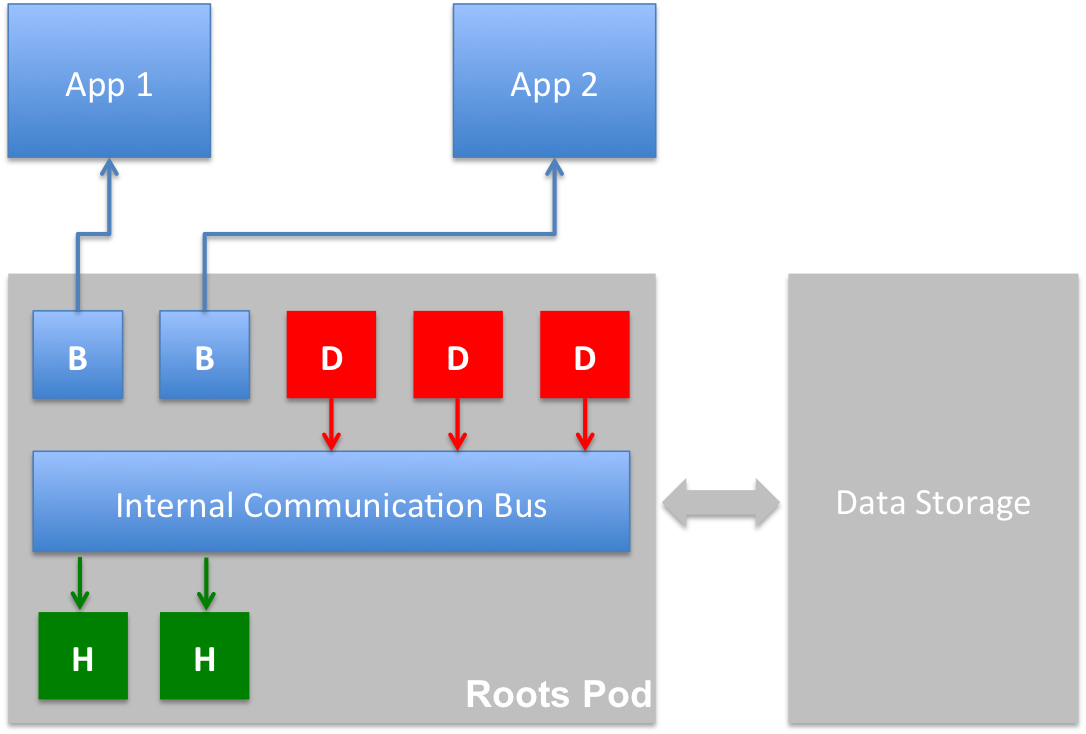
\includegraphics[scale=0.45]{roots_pod}
\caption{Anatomy of a Roots pod. The diagram shows 2 application benchmarking processes (B), 
3 anomaly detectors (D), and 2 handlers (H). Processes communicate via a shared
memory communication bus local to the pod.}
\label{fig:roots_pod}
\end{figure}
Most data collection activities in Roots can be treated as passive -- i.e. they
happen automatically as the applications receive and process requests in the cloud
platform. They do not require explicit scheduling or management. In contrast,
application benchmarking and data analysis are active processes that require
explicit scheduling and management.  This is achieved by grouping benchmarking
and data analysis processes into units called Roots pods. 

Each Roots pod is responsible for starting and maintaining a preconfigured set of
benchmarkers and data analysis processes (i.e. anomaly detectors and handlers). 
These processes are light enough, so as to pack a large number of them
into a single pod. Pods are self-contained entities, and there is no inter-communication
between pods. Processes in a pod can efficiently communicate with each other 
using shared memory, and call out to the central Roots data storage to retrieve 
collected performance data for analysis. 
%This enables starting and stopping 
%Roots pods with minimal impact on the overall monitoring system. 
Furthermore, pods
can be replicated for high availability, and application load can be distributed
among multiple pods for scalability.

Figure~\ref{fig:roots_pod} illustrates a Roots pod monitoring two applications.
It consists of two benchmarking processes, three anomaly detectors and 
two anomaly handlers. The anomaly detectors and handlers are shown communicating
via an internal shared memory communication bus. 

%To automate the process of managing pods, they can be tied into the core
%process management framework of the PaaS cloud. That way whenever the cloud
%platform initializes, a collection of pods can be started automatically.
%Application deployment process of the PaaS cloud can be augmented
%to register each new application with one of the available pods, so that the
%benchmarkers and anomaly detectors can start running on the application.
%Moreover, pods can be moved around or restarted as needed in response
%to errors and autoscaling events that occur in the cloud platform.


\section{Implementation}
\textcolor{blue}{This section shows that Roots is more than just a good idea.
Perhaps a figure showing the implementaion components and architecture would
help make that point stronger.}

We implemented a Roots prototype for the AppScale cloud
platform~\cite{6488671}. AppScale is an open source PaaS cloud, API compatible
with the popular Google App Engine (GAE) cloud platform~\cite{gae}.  Due to
the API compatibility, any application developed for GAE can be deployed and
executed on AppScale with no code changes. Since AppScale is open source
software, we were able to modify parts of its implementation to integrate the
Roots APM into it. AppScale also turned out to be a great test environment
since we could deploy it locally, and run a number of existing App Engine
applications on it.

We use ElasticSearch~\cite{elasticsearch} as the data storage component of our prototype. ElasticSearch is ideal 
for storing large volumes of structured and semi-structured data. It supports scalability and 
high availability via sharding and replication.
ElasticSearch continuously organizes and indexes data, making the information available 
for fast retrieval and efficient querying. Additionally it also provides
powerful data filtering and aggregation features, which greatly simplify the implementations of high-level
data analysis algorithms.

We configure AppScale's front-end server (based on Nginx) to tag all incoming application requests
with a unique identifier. This identifier is attached to the request as a custom HTTP header.
All data collecting agents in the cloud extract this identifier, and include it as an attribute
in all the events reported to ElasticSearch. This enables our prototype to aggregate events originating
from the same application.

We implement a number of data collecting agents in AppScale to gather runtime information
from all major components. These agents buffer data locally, and store them in ElasticSearch
in batches. For scraping server logs and storing the extracted entries in ElasticSearch,
we use the Logstash tool~\cite{logstash}. Logstash supports scraping a wide range of standard log formats (e.g. 
Apache HTTPD access logs), and other custom log formats can be supported via a simple configuration.
It also integrates naturally with ElasticSearch.
To capture the PaaS kernel invocation data, we augment AppScale's PaaS SDK implementation,
which is derived from the GAE PaaS SDK. More specifically we implement an agent that records
all PaaS SDK calls, and reports them to ElasticSearch asynchronously. 

Roots pods are implemented as standalone Java server processes. Threads are used to run benchmarkers,
anomaly detectors and handlers concurrently within each pod. Pods communicate with ElasticSearch via
REST calls, and many of the data analysis tasks such as filtering and aggregation are performed
in ElasticSearch itself. By doing so a lot of the heavy computations are offloaded to the 
ElasticSearch cluster, which is specifically designed for high-performance query processing
and analytics. Some of the more sophisticated statistical analysis tasks (e.g. change point detection, 
linear regression) are implemented in R language,
and the Java-based Roots pods integrate with R using the Rserve protocol~\cite{Urbanek03rserve--}.

\subsection{SLO-based Anomaly Detector}
We implement a performance SLO checker as the primary anomaly detector in Roots. This anomaly detector
allows application developers to specify simple performance SLOs for deployed applications. A
performance SLO consists of an upper bound on the application response time ($T$), and the probability ($p$)
that the application response time falls under the specified upper bound. Therefore, a general performance 
SLO can be stated as: ``application responds under $T$ milliseconds $p$\% of the time''.

When activated for a given application this anomaly detector starts a benchmarking process
that periodically measures the response time of the target application. The detector then periodically
analyzes the collected response time measurements to check if the application meets the specified performance
SLO. Whenever it detects that the application has failed to meet the SLO, it triggers an anomaly event. 
The SLO-based anomaly detector supports following configuration parameters:
\begin{itemize}
\item Performance SLO: Response time upper bound ($T$), and the probability ($p$).
\item Sampling rate: Rate at which the target application is benchmarked.
\item Analysis rate: Rate at which the anomaly detector checks whether the application has failed to meet the SLO.
\item Minimum samples: Minimum number of samples to collect before checking for SLO violations.
\item Window size: Length of the sliding window (in time) to consider when checking for SLO violations. This
acts as a limit on the number of samples to keep in memory.
\end{itemize}

Once the anomaly detector comes across an SLO violation, it will continue to see the violation
until the historical data which contains the anomaly drops off from the sliding window. 
In order to prevent the detector from needlessly reporting the same anomaly multiple times,
we purge all the data from anomaly detector's sliding window whenever it detects an SLO violation.
However, the detector cannot check for further SLO violations until it repopulates the sliding window 
with the minimum number of samples. This implies that each anomaly is followed by a ``warm up'' period.
For instance, with a sampling rate of 15 seconds, and a minimum
samples count of 100, the warm up period can last up to 25 minutes.

\subsection{Path Distribution Analyzer}

Path distribution analyzer is another special anomaly detector we implement in Roots. This
anomaly detector periodically analyzes the PaaS kernel invocations made by the applications.
By aggregating the PaaS kernel invocations by application request identifiers, and then sorting them by
their sequence numbers, this anomaly detector is able to identify the sequence of
PaaS kernel invocations made by each application request. 
Each identified invocation sequence corresponds to a path of
execution through the application code (i.e. a path through the control flow graph of the application). 
Then the anomaly detector evaluates the number of requests
that invoked the same PaaS kernel invocation sequence. From that the anomaly detector
computes the distribution of different execution paths of an application.

A path distribution is comprised of the set of execution paths available in an application, along
with the proportion of requests that executed each path.
It is an indicator of the type of request workload handled by an application.
For example consider a data management application that has a read-only execution path, and a read-write 
execution path. If 90\% of the requests execute the read-only path, and the remaining 10\% of the requests
execute the read-write path, we may characterize the request workload as mostly read-only. 
Roots path distribution analyzer facilitates computing the path distribution for each application
with no static analysis, by only analyzing the runtime data gathered from the applications.

Roots path distribution analyzer periodically computes the path distribution for a given application.
If it detects that the latest path distribution is significantly different from the distributions seen in the 
past, it triggers an anomaly. This is done by computing the mean request proportion for each path
(over a sliding window of historical data),
and then comparing the latest request proportion values against the means. If the latest proportion
is off by more than $n$ standard deviations from its mean, the detector considers it to be an
anomaly. The sensitivity of the detector can be configured by changing the value of $n$, which
defaults to 2. 

This anomaly detector enables developers to know when the nature of their application request
workload changes. For example in the previous data management application, if suddenly 90\%
of the requests start executing the read-write path, the Roots path distribution analyzer will
detect the change as an anomaly. Similarly it is also able to detect when new paths of execution
are being invoked by requests (a form of novelty detection).

\subsection{Workload Change Analyzer}
Performance anomalies can arise due to bottlenecks in the cloud platform or changes in the application
workload.
When Roots detects a performance anomaly (e.g. an application failing to meet its performance SLO),
we need to be able to determine which of the above two causes may be behind it.
To check if the workload of an application has changed recently, Roots uses a workload change analyzer.
This is implemented as an anomaly handler, which gets executed every time an anomaly detector
notifies of a performance anomaly. Note that this is different from the path distribution analyzer,
which is implemented as an anomaly detector. While the path distribution analyzer looks for changes in the
\textit{type} of the workload, the workload change analyzer looks for changes
in the workload \textit{size}. 
In other words, it determines if the target application has received more requests than usual, which
may have caused a performance degradation.

Workload change analyzer uses change point detection algorithms to analyze the historical trend of 
the application workload. We use the ``number of requests
per unit time'' as the metric of workload size. This information can be obtained from the Roots
data storage as a time series. Our implementation of Roots supports a number of well known change point
detection algorithms (PELT~\cite{doi:10.1080/01621459.2012.737745}, binary segmentation 
and CL method~\cite{chen1993joint}), any of which can be used to detect level shifts in the
workload size. Algorithms like PELT favor long lasting shifts (plateaus) in the workload trend, over momentary spikes.
We expect momentary spikes to be fairly common in workload data. But it's the plateaus that cause
request buffers to fill up, and hog server-side resources for extended periods of time thus
causing noticeable performance anomalies.

\subsection{Bottleneck Identification}
Now we describe our algorithm for identifying performance bottlenecks. It uses a combination
of quantile analysis, linear regression and change point detection. While Roots can
support many different bottleneck identification algorithms, we use
the algorithm proposed here in all of our experiments, and show that it produces accurate results nearly
100\% of the time. It has been carefully designed to identify the true bottleneck from a number
of candidates, and it is a major contribution associated with this work.

Applications running in the cloud consist of user code executed on the application server, 
and remote service calls to various PaaS kernel services. AppScale cloud
consists of the same kernel services present in the Google App Engine public cloud (datastore, memcache,
urlfetch, blobstore, user management etc.).
We consider each PaaS kernel invocation, and the code running on the application server as 
separate \textit{components}. Each application request causes one or more components to
execute, and any one of the components can become a bottleneck to cause performance anomalies.  
The purpose of bottleneck identification is to find, out of all
the components executed by an application, the one component that is most likely to have caused 
application performance to deteriorate.

Suppose an application makes $n$ PaaS kernel invocations ($X_1, X_2, ... X_n$) for each request. 
For any given application request,
Roots captures the time spent on each kernel invocation ($T_{X_1}, T_{X_2}, ... T_{X_n}$), and the 
total response time ($T_{total}$) of the request. These time values are related by the formula
$T_{total} = T_{X_1} + T_{X_2} + ... + T_{X_n} + r$, where $r$ is all the time spent in the resident 
application server executing user code. $r$ is not
directly measured in Roots, but it can be computed from the above formula 
since Roots captures $T_{total}$ and all other $T_{Xn}$ values. In our previous
work we have shown that PaaS-hosted web applications spend most of their time invoking PaaS kernel services.
Therefore we may state that $r \ll T_{X_1} + T_{X_2} + ... + T_{X_n}$.

Roots bottleneck identification mechanism selects up to four components as possible candidates
for the bottleneck. These four candidates are then further evaluated by a weighted algorithm to
determine the actual bottleneck in the cloud platform. We first describe how Roots selects the
bottleneck candidates.

\subsubsection{Relative Importance of PaaS Kernel Invocations} 
The purpose of this metric is to find the component that is contributing mostly towards the variance in the total
response time. We start by selecting a window $W$ in time which includes a sufficient number of application requests,
and ending at the point when the performance anomaly was detected. Note that for each application request
in $W$, we can fetch the total response time ($T_{total}$), and the time spent on individual PaaS kernel
services ($T_{X_n}$) from the Roots data storage.

Then we take all the $T_{total}$ values
and the corresponding $T_{X_n}$ values in $W$, and fit them to the linear regression model
$T_{total} = T_{X_1} + T_{X_2} + ... + T_{X_n}$. Here we leave $r$ out deliberately, since it is typically small. To prevent
any bad data from skewing the model, we also filter out requests where the $r$ value is too high. This
is done by computing the mean ($\mu_r$) and standard deviation ($\sigma_r$) of $r$ over the selected window, and removing 
any requests where $r > \mu_r + 1.65\sigma_r$.

Once the regression model has been computed, we run a relative importance algorithm~\cite{JSSv017i01} to rank each of the
regressors (i.e. $T_{X_n}$ values) based on their contribution to the variance of $T_{total}$. 
We use the LMG method~\cite{lmg80} which is resistant to multicollinearity, and provides a break down of the $R^2$ value of
the regression according to how strongly each regressor is influencing the variance of the dependent variable.
The relative importance values of the regressors add up to the $R^2$ of the linear regression. We consider
$1 - R^2$ (the portion of variance in $T_{total}$ not explained by the PaaS kernel invocations) as the relative importance of $r$. 
The component associated with the highest ranked regressor is a strong candidate
for the bottleneck that we are looking for. Statistically, this is the component that causes the application
response time to vary the most.

\subsubsection{Historical Trend of Relative Importance}
This is a simple extension of the previous metric. We divide the time window $W$ into equal-sized segments,
and compute the relative importance metrics for regressors within each segment. We also compute the
relative importance of $r$ within each segment. This way we can
obtain a time series of relative importance values for each regressor and $r$. These time series
represent how the relative importance of each component has changed over time.

We subject each time series to change point analysis to detect if the relative importance of any particular
variable has increased recently. If such a variable can be found, then the component
associated with that variable is also a potential candidate for the bottleneck. 
The candidate selected by this method represents is
a component whose performance has been stable in the past, and has become variable recently. 

\subsubsection{High Quantiles}
Next we turn our attention to the individual distributions of the $T_{X_n}$ and $r$. 
Recall that for each PaaS kernel invocation
$X_k$, we have a distribution of $T_{X_k}$ values in the window $W$. Similarly we
can also extract a distribution of $r$ values from $W$. Out of all the available distributions
we wish to find the one whose quantile values are the largest.
Specifically, we compute a high
quantile (e.g. 0.99 quantile) for each distribution. The component, whose distribution 
contains the largest quantile value
is chosen as another potential candidate for the bottleneck. This component can be considered
as taking a long time to execute in general.

\subsubsection{Tail End Values}
Finally, we further analyze each $T_{X_n}$ distribution and $r$ distribution to detect which one has the largest tail end values.
We are particularly interested in the values that are larger than a certain high quantile, such as the 0.99 quantile.
For each tail end value $t$, we compute the metric $P^q_t$. This is the percentage difference between $t$ and the
$q$ quantile of the corresponding distribution. The component, whose distribution distribution has
the largest $P^q_t$ is chosen as another potential performance bottleneck.
This is the case where a component has rare outliers which are much larger than the rest of 
the values in its distribution (i.e. point anomalies).

\subsubsection{Selecting the Performance Bottleneck}
Above four mechanisms can choose up to four candidates for the performance bottleneck. The number of
chosen candidates can be less than four, since the same candidate can get selected from more than
one mechanism. Note that each of the above four mechanisms are designed to look for different
types of bottlenecks. The relative importance method looks for a component that has consistently
high variance. The historical trend of relative importance facilitates finding a component whose
performance has only recently become highly variable. The high quantile method is good at
finding a component which is slow in general. The last method finds a component with poor
tail latency. If more than one of these methods choose the same candidate for the bottleneck,
we can claim it to the actual bottleneck with high confidence.

Based on the above intuition, we design a simple weighting mechanism to find the actual
bottleneck from the selected candidates. Any component chosen by the relative importance
method gets 4 points. Components chosen by the other three methods get 3 points each. 
We sum up the points assigned to each component, and the component with the highest
score is declared to be the bottleneck. The relative importance method acts as a tie breaker
in case the four methods select four different candidates. The performance anomalies we
are interested in are typically caused by long lasting performance issues in the system 
(pattern anomalies). Since the relative importance method looks for components with
consistently high variance, it is somewhat better at finding components
with lasting performance issues.


%
% The following two commands are all you need in the
% initial runs of your .tex file to
% produce the bibliography for the citations in your paper.
\bibliographystyle{abbrv}
\bibliography{sigproc}  % sigproc.bib is the name of the Bibliography in this case
% You must have a proper ".bib" file
%  and remember to run:
% latex bibtex latex latex
% to resolve all references
%
% ACM needs 'a single self-contained file'!
%
%APPENDICES are optional
%\balancecolumns

\end{document}
